\documentclass[letterpaper, 12pt, oneside]{memoir}
\usepackage{fontspec}

%%%%%%%%%%%%%%%%%%%%%%%%%%%%%%%%%%%%%%%%%%%%%%%%%%%%%%%%%%%%%%%%%%%%%%%%%%%%%%%
% BEG: PACKAGES
%
\usepackage{amsmath}
\usepackage{enumitem}
\usepackage{geometry}
\usepackage{graphicx}
\usepackage{hyperref}
\usepackage{tikz}
\usetikzlibrary{arrows.meta, calc, cd, fadings, positioning, shadings}
\usepackage{url}
\usepackage{xcolor}
% END: PACKAGES
%%%%%%%%%%%%%%%%%%%%%%%%%%%%%%%%%%%%%%%%%%%%%%%%%%%%%%%%%%%%%%%%%%%%%%%%%%%%%%%

%%%%%%%%%%%%%%%%%%%%%%%%%%%%%%%%%%%%%%%%%%%%%%%%%%%%%%%%%%%%%%%%%%%%%%%%%%%%%%%
% BEG: COLOR/TEXT/FONT CONFIGURATION
%

\setmainfont{SourceSerifPro-Regular}[
  BoldFont = SourceSerifPro-Bold,
  ItalicFont = SourceSerifPro-It,
]
\setsansfont{SourceSansPro-Regular}[
  BoldFont = SourceSansPro-Bold,
  ItalicFont = SourceSansPro-It,
]
\setmonofont{SourceCodePro-Regular}[
  BoldFont = SourceCodePro-Bold,
  ItalicFont = SourceCodePro-It,
  Scale = 0.90,
]

\definecolor{Orange}{cmyk}{0, 0.40, 0.80, 0}
\definecolor{RichBlack}{cmyk}{0.25, 0.25, 0.25, 0.70}

\tikzfading[name=fade lightly right,%
            left color=transparent!0,%
            middle color=transparent!0,%
            right color=transparent!25]

\tikzset{%
  block/.style={%
    rectangle,
    minimum width=0.5in,
    minimum height=2.5em,
    very thick,
    draw=RichBlack,
    rounded corners,
    font={},
    align=center%
  },
  annotate/.style={%
    font={\small},
  },
  summer/.style={%
    circle,
    minimum width=0.2in,
    minimum height=0.2in,
    thick,
    draw=RichBlack,
  },
  signal/.style={%
    color=RichBlack,
    very thick,
    line join=round,
    rounded corners=0.25em,
    shorten >=0.05em%
  },
  arrow/.style={-{Latex[length=0.5em]}}
}
%
% END: TEXT/FONT CONFIGURATION
%%%%%%%%%%%%%%%%%%%%%%%%%%%%%%%%%%%%%%%%%%%%%%%%%%%%%%%%%%%%%%%%%%%%%%%%%%%%%%%

%%%%%%%%%%%%%%%%%%%%%%%%%%%%%%%%%%%%%%%%%%%%%%%%%%%%%%%%%%%%%%%%%%%%%%%%%%%%%%%
% BEG: DOCUMENT CONFIGURATION
%

% Chapter Styling
\renewcommand{\chaptername}{Lab}
\chapterstyle{veelo}

%
% END: DOCUMENT CONFIGURATION
%%%%%%%%%%%%%%%%%%%%%%%%%%%%%%%%%%%%%%%%%%%%%%%%%%%%%%%%%%%%%%%%%%%%%%%%%%%%%%%

%%%%%%%%%%%%%%%%%%%%%%%%%%%%%%%%%%%%%%%%%%%%%%%%%%%%%%%%%%%%%%%%%%%%%%%%%%%%%%%
% BEG: DOCUMENT METADATA
%
\hypersetup{
  xetex,
  pdfauthor={Rollen S. D'Souza},
  pdftitle={ECE 380 --- Introduction to Feedback Control, Spring 2020, Lab Manual},
  pdfcreator={XeLaTeX with the HyperRef package.},
  breaklinks,
  plainpages=false,
  pdfversion=4,
  pdfduplex={DuplexFlipLongEdge},
  unicode=true,
  pdftoolbar=true,
  pdfmenubar=true,
  pdffitwindow=false,
  pdfstartview={FitH},
  pdfnewwindow=true,
  colorlinks=true,
  linkcolor=blue,
  citecolor=green,
  filecolor=magenta,
  urlcolor=cyan,
  linktocpage=true
}

%
% END: DOCUMENT METADATA
%%%%%%%%%%%%%%%%%%%%%%%%%%%%%%%%%%%%%%%%%%%%%%%%%%%%%%%%%%%%%%%%%%%%%%%%%%%%%%%

\begin{document}

%%%%%%%%%%%%%%%%%%%%%%%%%%%%%%%%%%%%%%%%%%%%%%%%%%%%%%%%%%%%%%%%%%%%%%%%%%%%%%%
% BEG: TITLE PAGE
\newgeometry{margin=0.5in, marginparsep=0in}
\thispagestyle{empty}
\begin{titlingpage}
\begin{tikzpicture}[remember picture, overlay, x=1in, y=1in]
  \node[inner sep=0pt, anchor=north west, scope fading=south] at (current page.north west) {%
    \includegraphics[%
      height = 9.5in,%
      trim = 300 20 0 50,
      clip%
    ]{images/STP-2-Mission-Landing}%
  };

  \node [at={($(current page.north west)+0.5*(1, 0)$)}] (A1) {};
  \node [at={($(current page.south west)+1.0*(1, 0)$)}] (A2) {};
  \node [at={($(current page.south west)+2.0*(0, 1)$)}] (B) {};
  \node [at={($(current page.south east)+0.5*(0, 1)$)}] (C) {};

  \fill [color={Orange}, path fading={fade lightly right}]
    (A1)
    rectangle
    (A2);

  \fill [color={RichBlack}]
    (current page.south west)
    rectangle
    (A1);
  \fill [color={RichBlack}]
    (current page.north west)
    --
    ($(current page.north west) + 1.0*(1, 0)$)
    --
    ($(current page.north west) - 1.0*(0, 1)$)
    --
    (current page.north west);
\end{tikzpicture}
\vfill
\begin{flushright}
{
  \rmfamily\HUGE\noindent
  \textbf{ECE 380 --- Intro to Feedback Control}\\
  Spring 2020\\
  Lab Manual
}
\end{flushright}
\begin{flushright}
{
  \rmfamily\Large\noindent
  Rollen S. D'Souza
}
\end{flushright}
\vspace{0.25in}
\end{titlingpage}

\restoregeometry

\pagebreak
% END: TITLE PAGE
%%%%%%%%%%%%%%%%%%%%%%%%%%%%%%%%%%%%%%%%%%%%%%%%%%%%%%%%%%%%%%%%%%%%%%%%%%%%%%%

%%%%%%%%%%%%%%%%%%%%%%%%%%%%%%%%%%%%%%%%%%%%%%%%%%%%%%%%%%%%%%%%%%%%%%%%%%%%%%%
% BEG: COPYRIGHT BS
%
\thispagestyle{empty}
\noindent\textcopyright 2020 Rollen S. D'Souza\\

\noindent
Cover page image captured by SpaceX\textregistered~on their
STP-2 Mission, licensed under the Creative Commons Non-Commercial 2.0. See
\href{https://www.flickr.com/photos/spacex/48129269942/}{here}
for original content. It is, of course, a photo of one of their self-landing
booster rockets attempting a landing. If you are interested, see the discussion
by Lars Blackmore on \emph{Autonomous Precision Landing of Space Rockets}
in
\href{http://www.larsblackmore.com/nae_bridge_2016.pdf}{this publication}. It
isn't very technical but you can find where to jump from there if you want a
little more technical content.

\pagebreak
% END: COPYRIGHT BS
%%%%%%%%%%%%%%%%%%%%%%%%%%%%%%%%%%%%%%%%%%%%%%%%%%%%%%%%%%%%%%%%%%%%%%%%%%%%%%%

\frontmatter

\tableofcontents*
\thispagestyle{empty}

%\listoffigures*
%\listoftables*

%%%%%%%%%%%%%%%%%%%%%%%%%%%%%%%%%%%%%%%%%%%%%%%%%%%%%%%%%%%%%%%%%%%%%%%%%%%%%%%
% BEG: INTRODUCTION
%
\chapter{Introduction}
Welcome to your remote lab for ECE 380, Introduction to Feedback Control.
The in-lab portion of this course was designed to give you a pseudo hands-on
feel for control using analog circuits. As this is a remotely delivered lab,
we no longer can provide you with the hands-on feel!

We persist. This lab is designed to run in MATLAB. You will engage
in understanding, developing, executing and analyzing Simulink
diagrams that model control systems. Every lab, though artificial, is
provided with brief motivation on how one can see this applied in a real
world problem. I hope this helps connect the abstract block diagrams of
Simulink with the real world.

Control systems is a very broad topic with a long history that even predates
the ideas discussed in this course. This course and lab covers the very basic
notion of control, the idea of the negative feedback loop, buttressed by
the mathematics of linear dynamical systems (Laplace theory).

\section{Logistics}
Please

\section{MATLAB and Simulink}
MATLAB is a desktop (or command line) numerical and symbolic
mathematics computing environment. We will not rely heavily on MATLAB
scripting itself and instead use Simulink. Simulink is a
package add-on to MATLAB that allows you to design and simulate
systems (physical or otherwise) using block diagrams like in
Figure~\ref{fig:intro:1}.
%
\begin{figure}
  \centering
  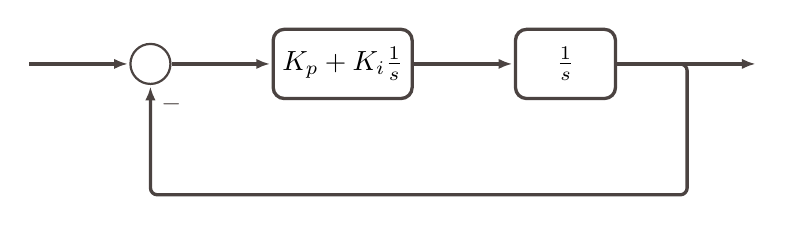
\begin{tikzpicture}[x=1in, y=1in]
    \node [draw, block] (Controller) {\(K_p + K_i\frac{1}{s}\)};
    \node [draw, block, right=0.5 of Controller] (Plant) {\(\frac{1}{s}\)};
    \node [draw, summer, left=0.5 of Controller] (Sum) {};
    \node [below=0.5 of Sum] (BelowSum) {};

    \draw [arrow, signal]
      (Controller.east) -- (Plant.west);
    \draw [arrow, signal]
      (Plant.east)
      --
      +(0.35, 0)
      |-
      (BelowSum.base)
      --
      (Sum.south)
      node [below right, annotate] {\(-\)};
    \draw [arrow, signal]
      (Sum.east) -- (Controller.west);
    \draw [arrow, signal]
      ($(Sum.west)+1*(-0.5, 0)$) -- (Sum.west);
    \draw [arrow, signal]
      (Plant.east) -- +(0.7, 0);
  \end{tikzpicture}
  \caption{
    Example feedback diagram. The blocks are differential equations, expressed
    as a Laplace transfer function, that take an input signal and produce an
    output signal.
  }
  \label{fig:intro:1}
\end{figure}
%
Figure~\ref{fig:intro:1} can be replicated perfectly in Simulink.
That fact makes it easy for engineers to quickly and easily design and verify
control designs. Simulink even supports direct interaction with
hardware but we will not utilize this feature.

The core of Simulink is the notion of a \emph{block}, maps that take an input
signal and produce an output signal.
The blocks we'll be concerned with primarily are \emph{gains}
(multiplier) depicted in Simulink like
\begin{center}
  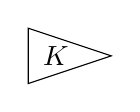
\begin{tikzpicture}[x=1em, y=1em]

    \draw
      (0, 0)
      --
      (3, 1)
      --
      (0, 2)
      --
      (0, 0)
      --
      (3, 1)
      node [at={(1, 1)}] {\(K\)};

  \end{tikzpicture}
\end{center}
and \emph{transfer functions} depicted in Simulink like
\begin{center}
  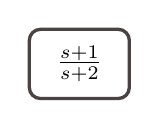
\begin{tikzpicture}[x=1em, y=1em]

    \node [draw, block] (Plant) {\(\frac{s+1}{s+2}\)};

  \end{tikzpicture}.
\end{center}
You will be provided template blocks to help you set up the Lab plant, the
system we wish to control, and it will be your task to analyze this block
design a controller, and implement it by linking up blocks to the plant
in the appropriate feedback architecture.

\section{Git Version Control}
We will be using the \texttt{git} version control system in tandem with
the Gitlab hosted on \url{git.uwaterloo.ca} to facilitate delivery of lab
content and to give you a mechanism for
\begin{enumerate}[label=(\arabic*)]
  \item{tracking your temporary work, and}
  \item{submitting your final work.}
\end{enumerate}
There is no requirement that you use git ``properly.'' If you are not
comfortable using the terminal to perform git operations, you can use graphical
tools like \href{https://www.sourcetreeapp.com/}{Sourcetree} or
\href{https://www.gitkraken.com/git-client}{GitKraken}. You can even manually
upload the files using the graphical web interface at \url{git.uwaterloo.ca}.
As long as your able to download files from your repository and upload your
solutions, I am happy. Having said that, it is an important skill in this
day and age to understand how to use version control. Therefore, this is a
great opportunity to learn git!


% END: INTRODUCTION
%%%%%%%%%%%%%%%%%%%%%%%%%%%%%%%%%%%%%%%%%%%%%%%%%%%%%%%%%%%%%%%%%%%%%%%%%%%%%%%

\mainmatter

\chapter{Familiarizing Yourself with Simulink}\label{Lab:1}
Low-pass filters are ubiquitous. They can be found in the hardware of
audio processing chips, or the software of image editing tools. As you may
recall from a course on Signals and Systems theory, a low-pass filter
is a system that, generally speaking, rejects high-frequency signals while
``passing through'' low-frequency signals. In this lab you will be asked
to analyze a low-pass filter block and determine its parameters. This is not
meant to be a difficult lab and is instead designed to give you a sense of the
lab format.


\section{Objectives}
The primary objectives of this lab are to
\begin{enumerate}[label=(\arabic*)]
  \item{
    Install MATLAB, Simulink and required toolboxes.
    Alternatively, connect remotely to
    \url{engterm.uwaterloo.ca} or any other lab computer of your choice
    that has MATLAB.
  }
  \item{
    Understand how to create a Simulink diagram and how to run
    a simulation.
  }
  \item{
    Understand how to log signals for future inspection and how to then
    make time-domain measurements.
  }
\end{enumerate}
Although the list of required deliverables is not very large, you should
spend your time exploring Simulink so as to reduce the amount of time
you spend on future labs. That is, of course, completely up to you.

\section{Experimental Procedure}

\subsection{Acquiring the Bandwidth in Time-Domain}

\subsection{Acquiring the Settling Time and Time Constant}

%%%%%%%%%%%%%%%%%%%%%%%%%%%%%%%%%%%%%%%%%%%%%%%%%%%%%%%%%%%%%%%%%%%%%%%%%%%%%%%
% BEG: APPENDIX

\appendix

\chapter{Simulink Basics}\label{App:Simulink}

% END: APPENDIX
%%%%%%%%%%%%%%%%%%%%%%%%%%%%%%%%%%%%%%%%%%%%%%%%%%%%%%%%%%%%%%%%%%%%%%%%%%%%%%%

\backmatter
\end{document}
